
\subsection{Firmware}

Tato kapitola rozebírá některá specifika vývoje firmwaru pro STM, v porovnání například s vývojem
softwaru pro PC.
Firmware musí být celkově dostatečně malý, aby se vešel do flash paměti STM (256 KB).
Také musí být relativně spolehlivý.

% Spolehlivost
\subsubsection{Spolehlivost}

% Alokace paměti - nebudeme používat dynamickou alokaci.
\paragraph{Alokace paměti}
Vzhledem k tomu, že od firmware se očekává, že poběží bez vypnutí dlouhou dobu, je potřeba aby
dodržoval některé invarianty.
Tyto invarianty by měly zaručovat, že firmware nepřestane fungovat svojí vlastní vinou.
Samozřejmě vždy se může stát, že přestane fungovat některá z hardwarových komponent.
Takové případy se ale nedají rozumně ošetřit a nezbyde nám nic jiného, než celý systém vypnout,
je-li to vůbec možné.
Chyba firmwaru by mohla být například ta, že se dostane do stavu kdy dojde paměť.
Tomuto stavu se dá poměrně snadno zabránit tak, že v žádné části firmwaru nebudeme používat
dynamickou alokaci paměti.
V našem případě by nepoužívání dynamické alokace paměti neměl být problém, protože o všech datech,
která v STM mohou být uložena, dokážeme předem určit jejich maximální velikost.

% Real-time vlastnosti
\paragraph{Real-time vlastnosti}
Real-time vlastností firmwaru máme na mysli tu skutečnost, že jsme teoreticky schopni spočítat nebo
naměřit délku maximální resp. minimální trvání každého tasku.
Mohli bychom například deklarovat, že \emph{GUI task} nesmí trvat déle než
100 ms.
Pomocí watchdog \cite{ReferenceManual} periferie bychom tuto maximální dobu trvání tasku snadno zajistili - v
případě, kdyby task trval déle, watchdog by celý systém resetoval.

Pro náš firmware jsou ale tyto vlastnosti nedůležité a tak nebudeme měřit dobu trvání jednotlivých
tasků, ani nastavovat watchdog.


% Programovací jazyk - C vs C++
\paragraph{Programovací jazyk}
Máme na výběr pouze mezi C a C++.
Nemá moc smysl omezovat se pouze na C, navíc v rámci GUI se nám objektová hierarchie včetně
virtuálních metod velice hodí.
% nepoužíváme STL
V rámci celé aplikace jsme se rozhodli nepoužívat typy z STL (C++ Standard Template Library), hodně z
těchto typů totiž ve svých vnitřnostech používá operátor \texttt{new}.
Mohli bychom si sice implementovat vlastní alokátor, který by měl povoleno alokovat paměť pouze
v inicializační fázi programu resp. po určitý časový úsek.
Po uplynutí inicializační fáze programu bychom alokování vypnuli a jakýkoli pokus o alokaci další
paměti by znamenal chybu.
Dodejme ještě, že množství alokované paměti po dobu inicializační fáze se dá spočítat při překladu
a tudíž se jedná de-facto pouze o statickou alokaci paměti, přestože v programu během inicializační
fáze používáme typy, které můžou volat operátor \texttt{new}.
Kvůli přílišné složitosti tohoto řešení se ale raději spokojíme s tím, že STL nebudeme používat vůbec.
Navíc by nám toto omezené používání \uv{dynamické alokace} paměti pouze během inicializační fáze
moc nepomohlo, protože nejvíc bychom to využili pravděpodobně při parsování HTTP zpráv a to už
inicializační fáze rozhodně není.

Na závěr řekněme, že C++ používáme jako \uv{C with classes} a nikde v programu nepoužíváme ani operátor
\texttt{new}, ani funkci \texttt{malloc}.

% nepoužívání dynamické alokace je nepraktické
Nemožnost používání dynamické alokace paměti nám ztěžuje práci - všude totiž musíme používat pole s
konstantní velikostí (některé z těchto velikostí jsou definovány v souboru \texttt{settings.hpp}, jinak
jsou definované přímo v typech, které je používají) a indexy do těchto polí, a navíc musíme kontrolovat
jestli pole nepřeteklo.
V drtivé většině těchto případů by bylo daleko snazší použít například \texttt{std::vector}.

Přestože nepoužíváme STL, přidá nám C++ další abstrakci, která nám usnadní~programování.

% Struktura
\subsubsection{Struktura}

\begin{figure}[tbh]\centering
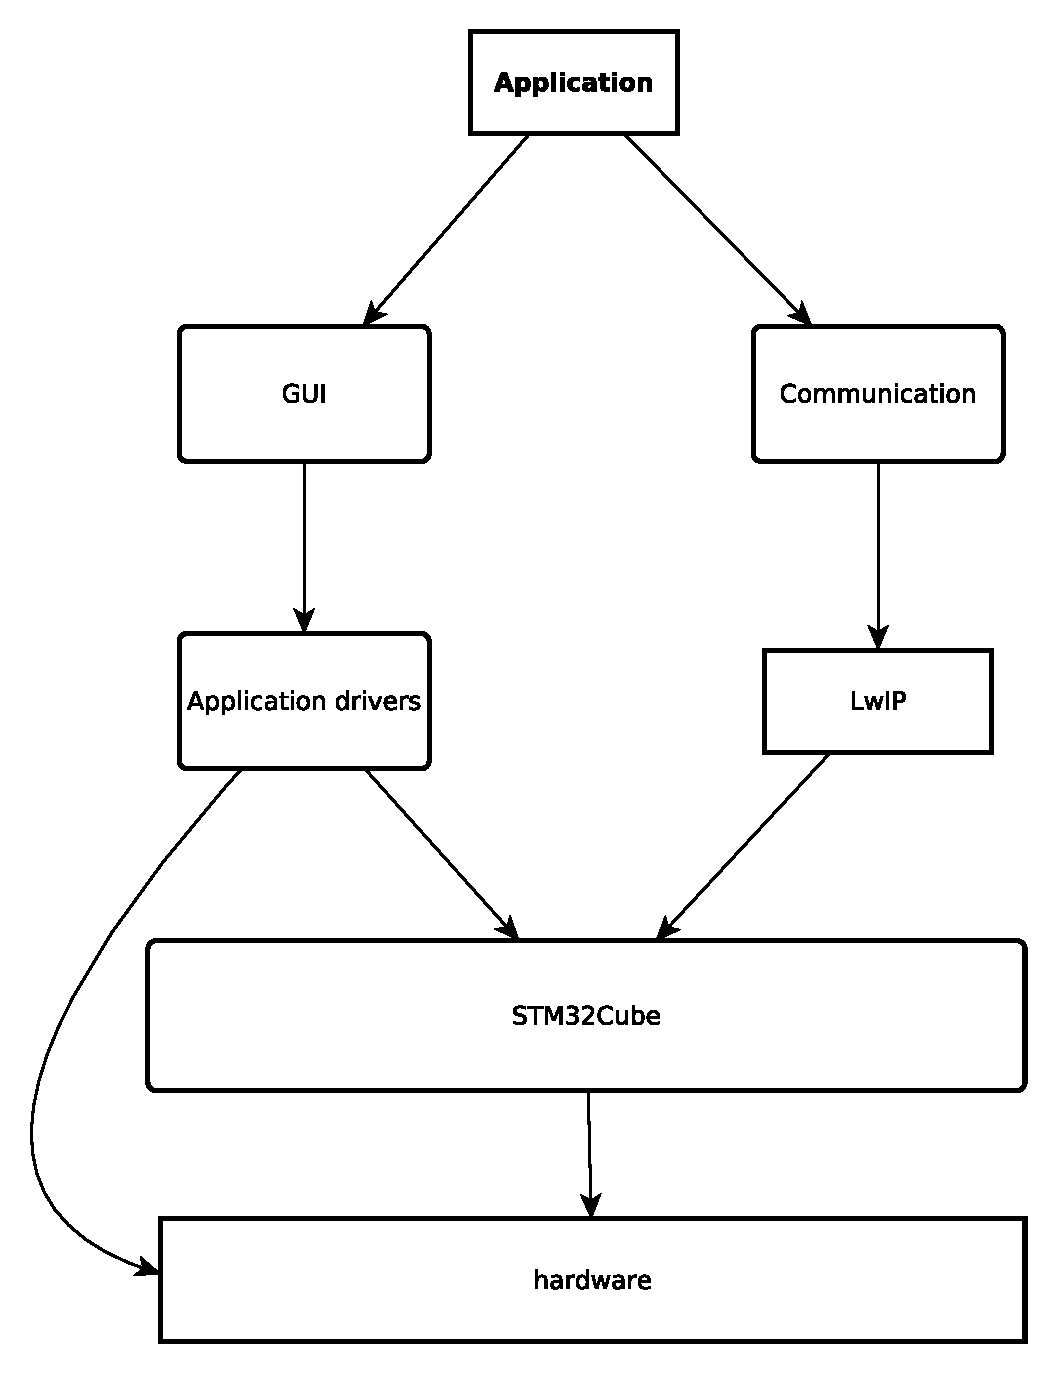
\includegraphics[width=140mm, height=140mm]{../diagrams/stm_fw_struktura.pdf}
\caption{Struktura firmware}
\label{stm-fw-struktura}
\end{figure}

% popis obrázku
Na obrázku \ref{stm-fw-struktura} vidíme strukturu celého firmware rozdělenou do jednotlivých vrstev.
Jednotlivé entity na obrázku odpovídají buď jednomu typu resp. třídě (jako je tomu v případě \texttt{Application}),
skupině tříd, nebo knihovně.
\texttt{Application} je na nejvyšší úrovni abstrakce a provádí hlavní aplikační logiku.
Jednak přímo pracuje se skupinou tříd \texttt{GUI}, pomocí které zobrazuje uživateli aktuální data,
případně mu umožňuje nastavení některých dat, ale také pracuje přímo se skupinou \texttt{Communication},
která obstarává veškerou komunikaci se serverem.
Skupina \texttt{Application Drivers} obsahuje aplikačně specifické wrappery hardwarových ovladačů nad
\texttt{STM32Cube}, v jednom případě i třídu \texttt{OneWire}, která přistupuje k hardware přímo
a ne přes \texttt{STM32Cube}.

Obrázek \ref{stm-fw-struktura} slouží pouze jako nástin struktury firmware a nikoli jako detailní popis
fungování jednotlivých typů.
Bližší informace o struktuře skupiny \texttt{Communication} je uvedena v kapitole \uv{Implementace komunikace},
struktura skupiny \texttt{GUI} je popsána v kapitole \uv{GUI}.

